\documentclass[tikz,border=2pt]{standalone}
\usepackage{amsmath,amssymb}
\usepackage{pgfplots}
\pgfplotsset{compat=1.18}

\begin{document}
% The quantile function reads the cdf backwards: for a probability u on the vertical axis,
% Q(u) is the smallest x whose cdf reaches u (here F is the logistic cdf, Q(0.8) = ln 4).
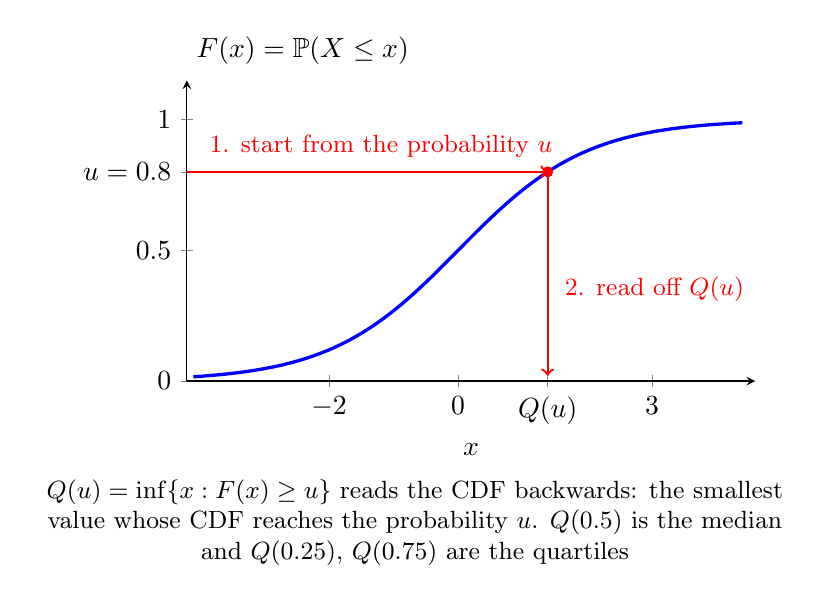
\begin{tikzpicture}
	\begin{axis}[
		axis lines=left, xmin=-4.2, xmax=4.6, ymin=0, ymax=1.15,
		xtick={-2,0,1.386,3}, xticklabels={$-2$,$0$,$Q(u)$,$3$}, ytick={0,0.5,0.8,1}, yticklabels={$0$,$0.5$,$u=0.8$,$1$},
		xlabel={$x$}, ylabel={$F(x)=\mathbb{P}(X\le x)$}, ylabel style={rotate=-90, anchor=south west, at={(axis description cs:0,1.02)}},
		samples=140, smooth, width=8.8cm, height=5.4cm, clip=false
		]
		\addplot[blue, very thick, domain=-4.1:4.4] {1/(1+exp(-x))};
		\draw[red, thick, ->] (axis cs:-4.2,0.8) -- (axis cs:1.386,0.8);
		\draw[red, thick, ->] (axis cs:1.386,0.8) -- (axis cs:1.386,0.02);
		\fill[red] (axis cs:1.386,0.8) circle (2pt);
		\node[red, font=\small, anchor=south west] at (axis cs:-4.0,0.82) {1. start from the probability $u$};
		\node[red, font=\small, anchor=west] at (axis cs:1.5,0.35) {2. read off $Q(u)$};
	\end{axis}
	\node[anchor=north, font=\small, align=flush center, text width=9.6cm] at ([yshift=-2pt]current axis.outer south) {$Q(u)=\inf\{x:F(x)\ge u\}$ reads the CDF backwards: the smallest value whose CDF reaches the probability $u$. $Q(0.5)$ is the median and $Q(0.25)$, $Q(0.75)$ are the quartiles};
\end{tikzpicture}
\end{document}
